%% 방법 논문 초안 v0.4의 한국어판(검토·공유용, 2026-10-19). 제출본은 영어 main_v0.4.tex. 이전 판: main_ko_v0.1.tex .. main_ko_v0.3.tex.
%% Overleaf: Main document = main_ko_v0.4.tex(zip 안에서는 main_ko.tex), Compiler = pdfLaTeX (한글 글꼴 오류 시 XeLaTeX).
\documentclass[twocolumn,10pt]{article}
\usepackage[letterpaper,margin=0.75in,columnsep=0.25in]{geometry}
\usepackage{kotex}
\usepackage[round]{natbib}
\usepackage{graphicx}
\usepackage{amsmath}
\usepackage{amssymb}
\usepackage{amsthm}
\usepackage{booktabs}
\usepackage{xcolor}
\usepackage[small]{caption}
\usepackage{url}
\usepackage{algorithm}
\usepackage{algpseudocode}

\newtheorem{proposition}{명제}
\newtheorem{lemma}{보조정리}
\newtheorem{assumption}{가정}
\newtheorem{definition}{정의}
\theoremstyle{remark}
\newtheorem{remark}{비고}

\newcommand{\todo}[1]{\textcolor{red}{[TODO: #1]}}
\newcommand{\tbd}{\textcolor{red}{TBD}}
\newcommand{\pilot}{\textsuperscript{\textcolor{gray}{$\dagger$}}}
\newcommand{\sg}{\operatorname{sg}}
\newcommand{\JS}{\operatorname{JS}}
\newcommand{\KL}{\operatorname{KL}}
\newcommand{\ours}{PGCT}
\floatname{algorithm}{알고리즘}

\title{Probe-Gated Critic Transfer:\\ 선택적 critic 공유를 위한 국소 팀원 추론\\ (다중 agent 강화학습)}
\author{익명 제출 (한국어판)}
\date{}

\begin{document}
\maketitle

\begin{abstract}
같은 환경을 쓰는 agent들이 서로 다른 목표의 팀에 속해 있어도, 누가 자기 팀원인지는 모를 수 있다. Probe-Gated Critic
Transfer(\ours{})에서 이웃한 agent들은 고정된 probe 관측 집합에 대한 행동 분포를 비교하고, 평활화한 Jensen--Shannon
divergence가 임계값보다 작은 이웃을 팀원으로 보고, 그 이웃의 critic을 probe 입력에서 distillation한다. 우리는 이 gate가 국소
팀 관계를 복원하는 조건(분리 마진이 추적 오차의 두 배보다 크다는 것, 그리고 측정 사이의 정책 변화로 정한 추적 오차의 상한)을
제시하고, 잘못된 donor가 만드는 편향의 상한을 구하며, 팀이 유도하는 결정 문제가 같으면 같은 입력에 대한 응답 비교로는 팀을
가를 수 없음을 보인다. 지금까지의 증거는 제한적이다. 팀 목표가 대칭인 4-agent 창고 과제에서 training seed 1개로는 \ours{}가
독립 PPO보다 평균 처리량이 높았다(6.4M step까지 episode당 배송 11.7 대 10.4). 그러나 gate는 다른 팀 agent끼리 연결했고, 같은
seed를 다시 돌리자 전이 방식들의 학습 시작 시점이 0.3--2.2M step 달라졌다. 고정 모델 오프라인 점검에서 정책 probe
divergence는 팀이 공간을 함께 쓰기 시작하면 팀을 가르지 못했고, checkpoint 사이 agent 자신의 응답 변화가 팀 신호만큼 컸다.
실제 방문 상태에서 질의한 보상 예측기는 독립적으로 학습된 계보에서도 팀을 갈랐으며(AUROC 0.71--0.79, 모델 3개), 그 신호는
주로 각 agent가 배운 자기 팀 보상에서 나왔다. 목표가 분리되고 팀 보상을 쓰는 6-agent 과제의 본 비교는 아직 하지 않았다.
\end{abstract}

\section{서론}
서로 다른 고객사의 창고 로봇, 서로 다른 운송사의 차량, 서로 다른 팀의 선수들은 공간은 함께 쓰지만 목표는 다르다. 집단 안에서
학습한 것(파라미터, 경험, 가치 추정)을 공유하는 것은 다중 agent 강화학습(MARL)에서 표본 효율을 높이는 흔한 방법이다
\cite{christianos2020seac,christianos2021seps}. 집단 사이에서는 같은 지식이 다른 목표를 나타낼 수 있다. 소속이 드러나 있지
않으면 agent는 세 가지 질문을 따로 마주한다. (Q1) 누가 내 팀원인가, (Q2) 누구의 critic이 내 학습을 돕는가, (Q3) Q1의 답은
언제 Q2의 좋은 답인가.

Q1에 대한 분산적인 답은 행동을 비교하는 것이다. 미리 합의한 같은 probe 관측을 평가하는 두 agent는 경험을 주고받지 않고도
행동 분포를 비교할 수 있다. Probe-Gated Critic Transfer(\ours{})가 이렇게 한다. 이웃들은 probe 응답의 평활화한
Jensen--Shannon(JS) divergence에 임계값을 적용하고, agent는 gate를 통과한 이웃의 critic을 distillation한다. 이것이 도움이
되려면 두 연결이 필요한데, 둘 다 일반적으로는 성립하지 않는다. 행동이 비슷하다고 목표가 같은 것은 아니다. 다른 목표가 같은
행동을 낳을 수 있고, 팀원이 다른 역할을 맡을 수 있으며, 학습 전 정책은 모두 비슷하고, 정책은 보상을 식별하지 못한다
\cite{ng2000irl}. 목표가 같다고 가치 함수가 호환되는 것도 아니다. 개인 보상에서는 팀원끼리 같은 과제를 두고 경쟁하고 숙련도도
다르다.

이 논문은 \ours{}를 설명하고, 두 연결이 언제 성립하는지 분석하고, 지금까지 측정한 결과를 방법에 불리한 결과까지 포함해 보고한다.
\ref{sec:analysis}절은 probe divergence의 성질, 팀을 정확히 국소 복원하는 조건과 정책 drift로 표현한 추정 오차 상한, 잘못된
donor가 만드는 편향의 상한, 정책 유사성과 가치 유사성을 가르는 반례, 같은 결정 문제를 마주한 팀의 식별 불가능성을 다룬다.
\ref{sec:setup}절은 시험 환경을 팀 식별 가능성과 팀원 critic의 호환성이라는 두 축에 놓고, donor 선택과 전이량을 분리하는
대조군을 둔다. \ref{sec:e1}--\ref{sec:main}절은 팀 대칭 과제의 seed 1개 실행, 고정 모델에서 probe 통계를 점검한 오프라인 감사,
아직 결과가 없는 본 실험의 설계를 보고한다. 이 초안의 학습 결과는 모두 seed 1개에서 나왔으므로 잠정적인 것으로 읽어야 한다.

\section{관련 연구}
\paragraph{선택적 공유.} SePS는 학습 전에 전이 데이터의 인코딩으로 agent를 군집화하고 군집 안에서 파라미터를 공유한다
\cite{christianos2021seps}. MADPS는 정책 사이 거리를 재서 파라미터 공유를 온라인으로 조정한다 \cite{hu2024madps}. HetDPS는 정책
이질성과 목표 이질성을 포함한 여러 이질성을 구분하고 그에 따라 공유한다 \cite{hu2026hetdps}. SEAC는 중요도 가중으로 경험을
공유한다 \cite{christianos2020seac}. 따라서 정책 거리로 공유 상대를 정하는 것 자체는 새롭지 않다. \ours{}는 세 가지 선택을
묶는다. 상대 선택은 중앙 군집화 없이 현재 통신 이웃 안에서 국소적·온라인으로 이루어지고, 정책은 공유 궤적이나 파라미터가 아니라
고정 probe 집합으로 비교하며, critic 예측만 전이하고 actor는 자기 경험으로 학습한다. 이 중 어느 하나도 새롭다고 주장하지
않으며, 이 조합이 언제 정당한지에 초점을 둔다.

\paragraph{분산 critic과 distillation.} Networked actor-critic은 통신 그래프 위에서 critic 파라미터를 합의로 모으며, 선형 함수
근사와 네트워크 평균 목적에서 수렴이 보장된다 \cite{zhang2018networked}. 이 보장은 개인 보상과 비선형 critic에는 그대로 적용되지
않는다. \ours{}는 probe 입력에서의 distillation으로 전이한다 \cite{rusu2016policy}.

\paragraph{팀원, 역할, 식별 가능성.} Ad hoc teamwork와 agent modelling은 관찰한 행동으로 다른 agent의 유형이나 정책을 추론한다
\cite{stone2010adhoc,albrecht2018modelling}. 역할 기반 MARL은 행동의 효과로 역할을 찾는다 \cite{wang2021rode}. 역할과 팀은
서로 다른 잠재 변수이며, 이 구분은 우리 결과에서 중요하다. 독립 PPO는 협력 MARL에서 강한 기준선이고
\cite{schulman2017ppo,dewitt2020ippo}, MAPPO는 중앙 critic을 더한다 \cite{yu2022mappo}. 정책이 보상을 결정하지 못한다는 것은
역강화학습의 고전적 결과이며 \cite{ng2000irl}, 우리의 식별 불가능성 결과는 그 팀 수준의 사례다. 결과 보고는
\cite{agarwal2021precipice}를 따른다.

\section{문제 설정}
\label{sec:setting}
agent $i\in\{1,\dots,N\}$, 관측 $o_i^t$, 행동 $a_i^t\in\mathcal{A}$, 보상 $r_i^t$를 갖는 부분 관측 확률 게임을 생각한다. 각
agent는 목표를 정하는 잠재 팀 $z_i\in\{1,\dots,K\}$에 속한다. 보상은 개인 보상이거나, 팀 보상 설정에서는 과제 보상이 과제를
완료한 팀의 모든 구성원에게 지급되고 shaping 항은 개인에게 남는다. agent는 자기 목표는 알지만 다른 agent의 $z_j$는 모른다. 통신
범위 안의 agent들이 시간에 따라 바뀌는 이웃 $\mathcal{N}_i(t)$를 이룬다. 학습 전에 모든 agent는 같은 probe 집합을 받고, 학습
중에 이웃끼리 probe 입력에 대한 행동 확률과 critic 예측을 주고받을 수 있다. 관측, 경험, 파라미터, 팀 라벨은 주고받지 않는다.
교환한 출력이 정책에 관한 정보를 일부 드러내므로 프라이버시는 주장하지 않는다. 각 agent는 PPO로 recurrent actor $\pi_i$와 critic
$V_i$를 학습한다.

\begin{definition}[국소 팀 관계]
시각 $t$에서 agent $i$의 국소 팀 관계는 $\mathcal{T}_i(t)=\{j\in\mathcal{N}_i(t): z_j=z_i\}$이다. 추정 $\hat{\mathcal{T}}_i(t)$가
$\mathcal{T}_i(t)$와 같으면 그 방법이 국소 팀 관계를 복원했다고 한다.
\end{definition}

\begin{definition}[전이 효용]
같은 학습 상태 $\Theta_n$에서 출발한 update 한 쌍, 즉 donor $j$를 쓰는 것과 전이하지 않는 것에 대해 전이 효용을
$U_{i\leftarrow j}=\mathbb{E}[J_i(\Theta^{i\leftarrow j}_{n,+})-J_i(\Theta^{i}_{n,+})]$로 둔다. $J_i$는 agent $i$의 평가 return이다.
Q1은 $\mathcal{T}_i$를, Q2는 $U_{i\leftarrow j}>0$인 donor를 묻는다.
\end{definition}

\section{Probe-Gated Critic Transfer}
\label{sec:method}
\paragraph{Probe 집합.} 모든 agent는 학습 전에 환경 배치에서 결정적 규칙으로 만든 단일 step 관측 집합
$\mathcal{Q}=\{q_m\}_{m=1}^{M}$을 똑같이 갖는다. probe는 recurrent 상태 0, 행동 mask 없이 평가하므로 질의 하나가 순전파 한 번이고
학습 궤적에는 영향을 주지 않는다.

\begin{assumption}[Probe 비교 가능성]
\label{as:comparability}
모든 probe $q_m$은 모든 agent에게 유효한 관측이고, 관측하는 agent 자신의 목표를 기준으로 상황을 모든 agent에게 같은 방식으로
나타낸다.
\end{assumption}
팀 상대 관측 채널을 쓰면 같은 텐서가 모든 agent에게 ``내 요청 선반''이나 ``내 목표''를 뜻한다. 다른 팀의 목표를 보여 주는
probe는 이 가정을 어기므로 만들 때부터 제외한다.

\paragraph{Probe divergence.} $p_i^m=\pi_i(\cdot\mid q_m,h=0)$이라 하자. $P$ update마다 이웃은 $\{p_i^m\}_m$을 교환하고 다음을
계산한다.
\begin{equation}
  D_{ij}=\frac{1}{M}\sum_{m=1}^{M}\JS(p_i^m,p_j^m),\quad
  \JS(p,q)=\tfrac12\KL(p\Vert\tfrac{p+q}{2})+\tfrac12\KL(q\Vert\tfrac{p+q}{2}).
  \label{eq:div}
\end{equation}
자연로그를 쓰므로 $D_{ij}\in[0,\ln 2]$이고 단위는 nat이다. $D_{ij}$는 JS divergence이고, 그 제곱근이 JS distance다.

\paragraph{평활화와 gate.} 첫 측정값으로 $\bar D_{ij}\gets D_{ij}$를 초기화하고, 이후 측정은 $i$와 $j$가 이웃일 때만
$\bar D_{ij}\gets(1-\beta)\bar D_{ij}+\beta D_{ij}$로 반영한다. 서로 범위를 벗어나면 $\bar D_{ij}$와 측정 횟수 $n_{ij}$는
유지하지만 전이는 하지 않는다. $U_0$ update의 warm-up 뒤에 agent $i$는 다음과 같이 추론한다.
\begin{equation}
  \hat{\mathcal{T}}_i(t)=\{j\in\mathcal{N}_i(t): n_{ij}\ge n_{\min},\ \bar D_{ij}<\tau\}.
\end{equation}

\paragraph{추론한 팀원의 critic distillation.} $j\in\hat{\mathcal{T}}_i(t)$에 대해 $\alpha_{ij}=1/|\hat{\mathcal{T}}_i(t)|$로 두고,
집합이 비어 있으면 peer 항을 두지 않는다. agent $i$는 다음을 최소화한다.
\begin{equation}
  \mathcal{L}_i=\mathcal{L}^{\mathrm{PPO}}_i+\lambda\sum_{j\in\hat{\mathcal{T}}_i(t)}\alpha_{ij}\,
  \frac{1}{M_{\mathrm{d}}}\sum_{m=1}^{M_{\mathrm{d}}}\big(V_i(q^{\mathrm{d}}_m)-\sg[V_j(q^{\mathrm{d}}_m)]\big)^2.
  \label{eq:loss}
\end{equation}
$\mathcal{L}^{\mathrm{PPO}}_i$는 PPO 손실(clip surrogate의 음수, value 손실의 $c$배, entropy 보너스의 음수)이고, $\sg$는
stop-gradient이며, donor 값은 update 시작 시점에 고정한다. 한 쌍의 두 방향이 같은 update에서 동시에 활성일 수 있고, 각
receiver는 상대의 update 전 값을 쓴다. 기본형은 probe 집합 자체에서 distillation한다. \ours{}-v2는 모든 과제 단계를 덮는 별도의
distillation 집합을 쓰고, 추론 집합에는 두 팀이 다르게 행동할 것으로 예상되는 상태만 둔다.

\paragraph{비용.} probe 한 회는 agent당 순전파 $M$번이고 쌍마다 확률 $M|\mathcal{A}|$개를 교환한다. 전이가 활성이면 값
$M_{\mathrm{d}}$개가 더해진다. $M=48$, $|\mathcal{A}|=5$, $P=5$, rollout 1{,}024 step이면 환경 5{,}120 step마다 쌍당 240개다.

\begin{algorithm}[t]
\caption{agent $i$의 \ours{}}
\label{alg:pgct}
\begin{algorithmic}[1]
\State $\pi_i,V_i$ 초기화; 모든 $j$에 대해 $\bar D_{ij}\gets$ 미정, $n_{ij}\gets 0$
\For{update $u=1,2,\dots$}
  \State $\pi_i$로 rollout 수집; 자기 보상으로 PPO target 계산
  \If{$u\bmod P=0$}
    \For{$j\in\mathcal{N}_i(t)$}
      \State $\mathcal{Q}$에서 $\{p^m\}$ 교환; $D_{ij}$ 계산(식~\ref{eq:div})
      \State $n_{ij}=0$이면 $\bar D_{ij}\gets D_{ij}$, 아니면 $(1-\beta)\bar D_{ij}+\beta D_{ij}$; $n_{ij}\gets n_{ij}+1$
    \EndFor
  \EndIf
  \State $u>U_0$이면 $\hat{\mathcal{T}}_i\gets\{j\in\mathcal{N}_i(t):n_{ij}\ge n_{\min},\bar D_{ij}<\tau\}$, 아니면 $\emptyset$
  \State $j\in\hat{\mathcal{T}}_i$로부터 update 전 $V_j(q^{\mathrm{d}}_m)$ 수신
  \State $\mathcal{L}_i$(식~\ref{eq:loss})로 $\pi_i,V_i$ update; $\hat{\mathcal{T}}_i=\emptyset$이면 peer 항 생략
\EndFor
\end{algorithmic}
\end{algorithm}

\section{분석}
\label{sec:analysis}
증명은 부록~\ref{app:proofs}에 있다. $\Delta(\mathcal{A})$는 행동 위의 확률 단체다.

\paragraph{Probe divergence.} JS divergence는 gate의 통계량일 뿐 gradient가 흐르지 않으므로, 필요한 것은 분포 공간에서의
성질이다.
\begin{proposition}[성질]
\label{prop:properties}
(a) $0\le D_{ij}\le\ln 2$, $D_{ij}=D_{ji}$이고, $D_{ij}=0$은 모든 $m$에서 $p_i^m=p_j^m$인 것과 동치다.
(b) $D_{ij}$는 $(\{p_i^m\}_m,\{p_j^m\}_m)$에 대해 결합 볼록이다.
(c) $d_{ij}=\sqrt{D_{ij}}$는 정책 위의 pseudometric이며, 특히 $d_{ik}\le d_{ij}+d_{jk}$이다.
\end{proposition}
\begin{remark}
$D_{ij}$는 네트워크 파라미터에 대해 볼록하지 않지만 최소화 대상이 아니므로 최적화에는 영향이 없다. gate의 불안정은 다른
종류다. 고정 임계값 때문에 donor 집합이 $\bar D_{ij}$의 불연속 함수가 되고, $\tau$ 근처의 추정값은 연속한 update 사이에서
gate를 뒤집을 수 있다. 명제~\ref{prop:recovery}와 \ref{prop:tracking}은 이것이 추론한 관계를 바꿀 수 없는 조건을 준다. (c)는
근사적 추이성을 준다. $i$가 $j$와 가깝고 $j$가 $k$와 가까우면 $i$도 $k$와 가깝다.
\end{remark}

\paragraph{임계값은 언제 팀을 복원하는가.}
\begin{assumption}[분리]
\label{as:separation}
update $n$에서 현재 이웃 쌍에 대한 $\delta_{\mathrm{in}}(n)=\max_{z_i=z_j}D_{ij}(n)$, $\delta_{\mathrm{out}}(n)=\min_{z_i\ne z_j}D_{ij}(n)$이
$\Delta(n)=\delta_{\mathrm{out}}(n)-\delta_{\mathrm{in}}(n)>0$을 만족한다.
\end{assumption}
\begin{proposition}[정확한 국소 복원]
\label{prop:recovery}
가정~\ref{as:separation} 아래에서 모든 이웃 쌍에 대해 $|\bar D_{ij}(n)-D_{ij}(n)|\le\epsilon$, $2\epsilon<\Delta(n)$,
$\tau\in(\delta_{\mathrm{in}}+\epsilon,\delta_{\mathrm{out}}-\epsilon)$이고 warm-up과 최소 측정 횟수를 채우면, 모든 $i$에 대해
$\hat{\mathcal{T}}_i(n)=\mathcal{T}_i(n)$이다. 이때 추론한 관계는 대칭이고 잘못된 donor는 쓰이지 않는다.
\end{proposition}
명제 자체는 간단하다. 쓸모는 측정해야 할 두 양, 마진 $\Delta$와 오차 $\epsilon$을 지목한다는 데 있다. probe 응답은 결정적이므로
$\epsilon$은 표본 잡음이 아니라 측정 사이에 정책이 바뀌는데 평균이 뒤따라가지 못해 생긴다.
\begin{lemma}[Drift]
\label{lem:drift}
연속한 두 측정 사이에 $i$와 $j$의 모든 probe 응답이 대칭 KL로 $\kappa$ 이하만 바뀌면, 즉 $\KL(p\Vert p')+\KL(p'\Vert p)\le\kappa$이면,
$|d_{ij}'-d_{ij}|\le\sqrt{\kappa}$이고 $|D_{ij}'-D_{ij}|\le2\sqrt{\kappa\ln 2}$이다.
\end{lemma}
\begin{proposition}[추적 오차]
\label{prop:tracking}
쌍의 모든 측정에서 $|D_{ij}(n)-D_{ij}(n-1)|\le\rho$이면, 첫 측정으로 초기화한 평활 추정은
$|\bar D_{ij}(n)-D_{ij}(n)|\le\frac{1-\beta}{\beta}\rho$를 만족한다. 따라서 $2\frac{1-\beta}{\beta}\rho<\Delta(n)$이면
명제~\ref{prop:recovery}가 적용된다.
\end{proposition}
PPO의 clip 목적은 방문 상태에서 update당 KL을 작게 유지하므로 $\kappa$가 작으리라고 기대할 수 있지만, probe 입력에서의 KL을
제한하지는 않는다. 보조정리~\ref{lem:drift}는 충분조건이고, $\rho$와 $\Delta$는 측정해야 한다. 측정 결과는 \ref{sec:audit}절에
있다. $\beta=0.35$이면 $(1-\beta)/\beta$는 $1.86$이다. $\beta$가 크면 빨리 따라가지만 평균 효과는 줄어든다. 임계값을 두 개 두는
히스테리시스가 gate 깜빡임의 표준적인 대책이다.

\paragraph{잘못된 donor의 비용.} 한 probe 입력 $q$에서 critic을 자유 출력 $v$로 이상화하고, 국소 회귀 target을 $y$(예: receiver
자신의 return 추정), donor 값을 $v_j$로 둔다.
\begin{proposition}[출력 공간에서의 distillation]
\label{prop:bias}
$\sum_j\alpha_{ij}=1$일 때 $f(v)=c(v-y)^2+\lambda\sum_j\alpha_{ij}(v-v_j)^2$는 $2(c+\lambda)$-강볼록이고 최소점은
$v^\star=\frac{cy+\lambda\sum_j\alpha_{ij}v_j}{c+\lambda}$이다. $\hat{\mathcal{T}}_i$의 donor가 $z_j=z_i$이면 $|v_j-y|\le\eta$,
아니면 $|v_j-y|\le\Gamma$를 만족하고 잘못된 donor의 가중치 합이 $a_{\mathrm{w}}$이면
$|v^\star-y|\le\frac{\lambda}{c+\lambda}\big((1-a_{\mathrm{w}})\eta+a_{\mathrm{w}}\Gamma\big)$이다.
\end{proposition}
$c=0.5$, $\lambda=0.01$이면 $\lambda/(c+\lambda)$는 약 $0.02$이고, 명제~\ref{prop:recovery}가 성립하면 $a_{\mathrm{w}}=0$이다. 이
이상화는 네트워크가 입력들 사이에 파라미터를 공유한다는 점과, $c$가 probe가 아니라 rollout 상태에 걸린다는 점을 무시한다.
파라미터 공간에서는 $\langle\nabla\mathcal{L}^V_i,\nabla\mathcal{L}^D_{i\leftarrow j}\rangle<0$일 때 peer 항이 value 손실과 충돌할 수
있다. 이것은 아직 측정하지 않았다 \todo{gradient 정렬 진단}.

\paragraph{팀 관계는 언제 호환성의 좋은 대리 지표인가.}
\begin{proposition}[정책 유사성은 가치 유사성을 제한하지 않는다]
\label{prop:counter}
모든 probe에서 $D_{ij}=0$이면서 $|V_i-V_j|=1/(1-\gamma)$인 두 agent가 있다.
\end{proposition}
반례는 자명하지만, Q1이 Q2에 답하지 못하며 호환성은 따로 재야 한다는 점을 분명히 한다.

\paragraph{팀은 애초에 식별 가능한가.} 다른 agent들의 정책을 고정하면 agent $i$는 자기 관측 위의 단일 agent 결정 문제를
마주한다. 기억 없는 관측-행동 사상 $\mu$ 모두에 대해, $i$가 $\mu$로 행동할 때 겪는 관측--보상 열의 분포가 $j$가 $\mu$로 행동할
때 겪는 분포와 같으면, $i$와 $j$의 문제가 \emph{일치한다}고 한다.
\begin{proposition}[팀 불변 결정 문제에서의 식별 불가능성]
\label{prop:nonid}
다른 팀 agent들에게 유도되는 결정 문제가 관측의 함수로서 일치하면, 기억 없는 정책 범위에서 한 팀에 최적인 관측-행동 사상은
다른 팀에도 최적이다. 최적 사상이 유일하면 목표에 최적인 정책들은 모든 쌍에서 $D_{ij}=0$을 만족하므로 $\Delta=0$이고, 어떤
임계값도 팀을 가르지 못한다. 그때 probe 응답의 차이는 역할이나 학습 진행 같은 다른 요인을 반영한다.
\end{proposition}
팀 상대 관측과 거울 대칭 과제가 함께 있으면 정확히 이 경우가 된다. 관측에 팀과 무관한 의미의 양(예: agent의 절대 위치)이 있고
팀의 목표가 다르면 유도된 문제가 달라지므로 명제가 적용되지 않는다.
\begin{remark}
\label{rem:reward}
논증은 비교하는 양이 관측과 행동의 함수라는 점만 쓴다. 따라서 공유 입력에서 질의하는 학습된 보상 모델 $\hat r_i(o,a)$에도 똑같이
적용된다. 두 팀의 보상이 팀 상대 관측의 같은 함수라면 정확한 보상 모델도 팀을 가르지 못한다. 질의 집합이 이 경우를 피하는지는
보상이 팀에 따라 달라지는 질의의 수를 세어 확인할 수 있다(\ref{sec:audit}절).
\end{remark}

\section{실험 설계}
\label{sec:setup}
\paragraph{환경 계열.} 다중 로봇 창고 \cite{papoudakis2021benchmarking}의 2팀 변형을 쓴다. 관측은 팀 상대 채널(``내 요청
선반'', ``내 목표'')을 가진 자기 중심 $11\times11$ 의미 격자와, 절대 위치를 포함한 ego feature다. 팀의 요청 선반은 절반이 상대
팀 쪽 절반에 놓이도록 뽑는다. 아래 과제는 모두 무작위 초기화에서 학습하며, 같은 seed에서는 모든 방법이 비트 단위로 같은
가중치에서 출발하고 donor 집합만 다르다.

\paragraph{E1(팀 대칭 대조 조건).} $11\times10$ 맵, agent 4명(agent 1·3은 빨강 팀, 2·4는 파랑 팀), 팀당 요청 선반 2개, 아래
가운데에 붙어 있는 두 목표, 개인 보상, 센서·통신 범위 5. 팀 상대 채널 때문에 두 팀이 같은 결정 문제를 마주하므로
명제~\ref{prop:nonid}는 팀을 식별할 수 없다고 예측한다. E1은 찾을 팀이 없을 때 방법이 해를 끼치는지를 시험할 뿐, 팀원 추론을
시험할 수는 없다.

\paragraph{E1-F(목표 분리, 개인 보상).} E1과 같지만 목표가 아래 양 모서리에 있어, 목표에서 먼 곳에서 선반을 든 agent는 팀마다
다른 방향을 골라야 한다. 다섯 방법의 첫 실행은 약 1.7M step에서, 어느 방법도 안정적으로 배송하기 전에 중단됐고 재개하지
않았다(\ref{sec:main}절). E1-F를 바꾼 이유는 셋이다. 학습이 느렸다. 개인 보상에 팀당 요청 2개라 팀원끼리 같은 과제를 두고
경쟁하므로 ``팀원이 좋은 donor''라는 전제가 약해진다. agent가 4명이라 seed당 팀원 쌍이 2개뿐이다.

\paragraph{B(본 과제, 목표 분리, 팀 보상).} $11\times10$ 맵, 3명씩 두 팀의 agent 6명, 팀당 요청 선반 3개, 아래 양 모서리의 목표,
팀 보상, 센서 범위 5, 통신 범위 3. 무작위 정책에서 agent의 평균 이웃 수는 1.36이고, 23\%의 step에서는 이웃이 없으며, 44\%의
step에서는 범위 안에 팀원이 한 명 이상 있다. 전이는 국소적이지만 드물지는 않다. 짝수 seed에서는 목표 좌우를 바꾼다. 이것은
좌우 배치에 대한 강건성 시험이다. 한 seed 안에서는 여전히 팀과 방향이 일치하므로, 팀원 추론과 방향 선호를 분리하지는 않는다.
표~\ref{tab:axes}는 과제들을 분석의 두 축에 놓는다. 대안 과제 두 개를 미리 정해 두었다. A(E1-F에 팀 보상)와 C(B를
$11\times16$ 맵으로 넓힌 것)다. 과제는 IPPO pilot(2M step, 과제당 seed 2개)에서 IPPO가 배송을 시작하는지만으로 고르며, probe나
전이 결과는 기준으로 쓰지 않는다 \todo{pilot 결과; B, A, C 중 선택}.

\begin{table}[t]
\centering
\small
\resizebox{\columnwidth}{!}{%
\begin{tabular}{lcc}
\toprule
 & 팀원 critic 호환 & 호환 안 됨 / 불명 \\
\midrule
행동으로 팀 식별 가능 & B, A(팀 보상; 예상) & E1-F(개인 보상) \\
식별 불가능 & -- & E1(측정) \\
\bottomrule
\end{tabular}}
\caption{분석의 두 축에 놓은 과제. E1: 명제~\ref{prop:nonid}로 식별 가능성이 배제되고, 고정된 커리큘럼 모델에서는 팀원보다
다른 팀 agent의 critic과 섞을 때 더 도움이 됐다. E1-F, B, A: 목표 배치상 식별 가능할 것으로 예상하며 호환성은 측정 예정이다
\todo{측정 후 B 위치 확정}.}
\label{tab:axes}
\end{table}

\paragraph{Probe 집합.} canonical 집합은 pickup, 배송, 반납을 덮는 상태 48개다. v2 추론 집합은 agent가 요청 선반을 들고 있고 어느
팀의 목표도 보이지 않는 상태 48개라, 입력이 모든 agent에게 유효하고(가정~\ref{as:comparability}) 올바른 행동은 자기 팀이 어디로
배송하는지에 달려 있다. v2 distillation 집합은 과제 단계별로 균형을 맞춘 상태 64개다. 모든 probe는 학습 환경에서 실제로 구현해
확인했다.

\paragraph{방법.} IPPO(전이 없음), All-peer(모든 이웃이 donor), Oracle-team(이웃 중 실제 팀원, 상한이 아니라 특권 정보를 쓴 참조),
\ours{}, \ours{}-v2. Random-gated 전이는 donor 선택과 전이량을 분리한다. 매 update마다 참조 \ours{} 실행이 그 update에 실제로 쓴
방향 arc 수만큼을 현재 통신 이웃 중에서 균등하게 뽑고, receiver별 가중치 합은 1이며, 채우지 못한 arc는 다음 update로 넘긴다.
구현과 smoke 시험은 마쳤고, 중단된 E1-F \ours{} 실행의 이웃 그래프 위에서 재생하면 목표 arc 8{,}686개를 모두 썼다. 전이량을 맞춘
Oracle은 계획 중이다 \todo{구현}. \ours{}의 설정은 $P=5$, $\beta=0.35$, $\tau=0.12$ nats, $U_0=100$, $n_{\min}=8$,
$\lambda=0.01$, $c=0.5$다(부록~\ref{app:hyper}). 팀 보상에서는 팀원이 같은 step에 보상을 받으므로, agent가 보상 기록을 교환할 수
있다면 그 동시성만으로 팀이 드러난다. 그래서 이런 정보가 무엇을 주는지의 참조로 보상 상관 기준선(보상 기록의 상관, 큰 보상
사건의 상관, 사건 step의 Jaccard 겹침)을 보고하고, probe 통계를 이것과 비교한다.

\paragraph{지표.} \emph{학습}: 배송 시작 시점(episode당 배송 1 이상인 평가가 처음으로 세 번 연속된 시점의 첫 평가), 학습 중
episode당 평균 배송, 최종 배송(마지막 평가 5회), 배송을 배운 agent 수. 보상의 첫 발견 시점이 실행마다 크게 달라지므로
(\ref{sec:e1}절), 시작 시점부터 episode당 배송 $k$에 이르기까지의 시간 $\Delta T_k$를 보조 지표로 함께 보고한다. \emph{추론}:
실제 전이 arc 중 팀 내부 arc의 비율을 같은 이웃 그래프에서의 우연 수준인 Random-gated의 비율과 비교한다. 그 밖에
$\hat{\mathcal{T}}_i$의 정밀도·재현율, checkpoint에서 $D_{ij}$의 같은 팀 AUROC, 실측 마진 $\Delta$와 drift $\rho$를 본다.
\emph{호환성}: receiver의 critic을 팀원의 critic과 섞을 때와 다른 팀 agent의 critic과 섞을 때 가치 오차가 얼마나 줄어드는지를
비교한다. 평가는 51{,}200 step마다 고정 reset seed로 deterministic masked 정책 20 episode×500 step이다. 본 과제에서는 방법당
training seed 5개 이상을 계획한다 \todo{seed}.

\paragraph{결과 해석 기준.} 본 과제를 돌리기 전에 해석을 정해 두었다. \ours{}가 Random-gated 수준보다 팀원을 더 고르고
Oracle-team이 Random-gated보다 빨리 배우면 원래 설계를 유지한다. 팀원을 고르지 못하지만 Oracle-team이 도움이 되면 추론 단계를
고쳐야 한다. 팀원을 고르지만 Oracle-team이 도움이 되지 않으면 critic 공유 방식이나 ``팀원이 좋은 donor''라는 전제를 다시 봐야
한다. 둘 다 아니면 과제와 핵심 가정을 함께 다시 검토한다.

\section{팀 대칭 과제의 결과}
\label{sec:e1}
E1은 seed 1개로 학습했고 6.5M step에서 멈췄다. 통계는 공통 구간 6.4M step 기준이다(\pilot 표시). 같은 seed와 초기 가중치로
돌린 이전 실행이 약 2.5M step에서 중단됐는데, 이것은 두 번째 seed가 아니라 실행 간 변동을 보여 주는 용도로만 쓴다.

\begin{table}[t]
\centering
\small
\resizebox{\columnwidth}{!}{%
\begin{tabular}{lccccc}
\toprule
방법 & 시작 & 시작(반복) & 평균$\uparrow$ & 최종$\uparrow$ & 학습 \\
\midrule
IPPO & 2.05M & 2.05M & 10.4 & 23.2 $\pm$ 1.1 & 2/4 \\
All-peer & 3.94M & 1.79M & 3.7 & 19.4 $\pm$ 1.6 & 4/4 \\
Random-gated & \tbd & -- & \tbd & \tbd & \tbd \\
\ours{} & 1.74M & 2.10M & 11.7 & 27.3 $\pm$ 1.4 & 3/4 \\
\midrule
Oracle-team & 1.59M & 1.89M & 13.2 & 32.2 $\pm$ 1.7 & 3/4 \\
\bottomrule
\end{tabular}}
\caption{E1(팀 대칭), seed 1개\pilot, 공통 구간 6.4M step. 시작: episode당 배송 1 이상인 평가가 세 번 연속된 첫 시점.
시작(반복): 같은 seed·초기 가중치로 2.5M step에서 중단된 이전 실행. 평균: 6.4M까지 평가의 episode당 배송 평균. 최종: 마지막
평가 5회의 평균 $\pm$ 표준편차(seed 간이 아님). 학습: 마지막에 episode당 배송 1 이상인 agent 수.}
\label{tab:e1}
\end{table}

\begin{figure}[t]
\centering
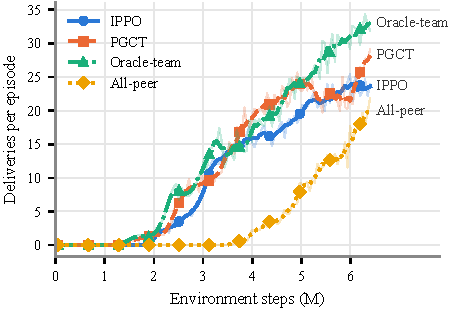
\includegraphics[width=\columnwidth]{figures/fig1_learning_curves.pdf}
\caption{E1의 평가 episode당 배송(seed 1개\pilot). 가는 선: 원 평가값, 굵은 선: 가운데 5점 이동평균.}
\label{fig:curves}
\end{figure}

\paragraph{학습.} 이 실행에서 \ours{}는 IPPO보다 평균 배송이 많았고(episode당 11.7 대 10.4, 약 12\%), 마지막에도
많았으며(27.3 대 23.2, 약 18\%), episode당 배송 20에 가장 먼저 도달했다(4.15M step; Oracle-team 4.66M, IPPO 5.07M; 표~\ref{tab:e1},
그림~\ref{fig:curves}). All-peer가 가장 늦게 시작했다. agent별로 보면(부록~\ref{app:e1}) IPPO는 팀마다 배송자를 한 명씩
학습시켰고, \ours{}와 Oracle-team은 세 번째 agent를, All-peer는 늦었지만 네 명 모두를 학습시켰다. 이 차이들은 seed 1개로 판별할
수 있는 범위 안에 있다. 반복 실행은 IPPO를 2.46M step까지 정확히 재현했지만, 전이 방식은 모두 1.4--1.6M step 이후 갈라졌다.
전이 경로의 비결정적 연산 때문으로 추정한다(부록~\ref{app:e1}). 반복 실행에서는 \ours{}의 시작 시점이 IPPO보다 앞서지 않고
뒤였고, All-peer의 시작 시점은 2M step 넘게 움직였다. 시작 시점부터 잰 속도의 순위는 기준에 따라 바뀐다. $\Delta T_5$는
\ours{} 0.77M, IPPO 0.82M, $\Delta T_{10}$은 1.54M과 1.13M, $\Delta T_{20}$은 2.41M과 3.02M이다. 따라서 E1에서 \ours{}가 IPPO보다
빨리 배운다고 주장하지 않는다. \ours{}와 Oracle-team에서 세 번째 agent가 늦게 배운 것은, 숙련된 agent의 critic을 distillation하면
스스로는 보상을 거의 못 받는 agent도 학습 신호를 얻는다는 가설과 맞는다. 이를 확인하려면 그 agent로의 전이를 막는 개입 실험이
필요하다 \todo{개입 실험}.

\begin{figure*}[t]
\centering
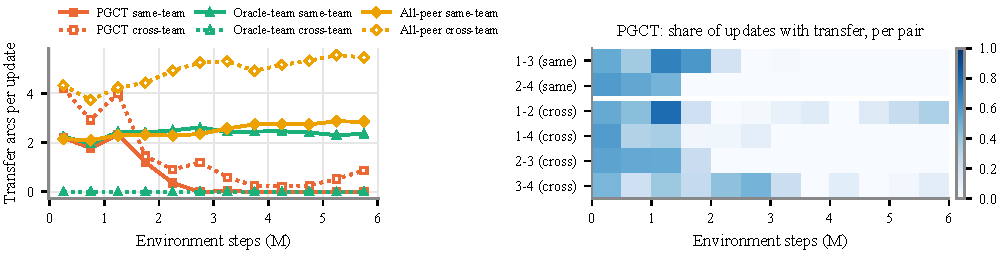
\includegraphics[width=\textwidth]{figures/fig3_critic_transfer.pdf}
\caption{E1의 실제 critic 전이(seed 1개\pilot). 왼쪽: 0.5M step 구간별 update당 팀 내부(실선)·팀 간(점선) 방향 전이 arc 수.
오른쪽: \ours{}에서 각 쌍이 critic 정보를 주고받은 update의 비율.}
\label{fig:transfer}
\end{figure*}

\paragraph{추론.} 명제~\ref{prop:nonid}는 E1에서 팀을 식별할 수 없다고 예측하며, 데이터도 그렇다. 3M step 이후 네 방법 모두
대부분의 checkpoint에서 팀원 사이 probe divergence가 다른 팀 agent 사이보다 컸다(부록~\ref{app:e1}). 즉 실측 마진이 음수였다.
4M step 이후 \ours{} 전이 arc의 95\%가 다른 팀 agent를 이었고(update당 팀 내부 0.03, 팀 간 0.63; 그림~\ref{fig:transfer}), 주로
같은 역할, 즉 자기 쪽 절반에 머무는 agent끼리 또는 상대 쪽 절반에서 선반을 가져오는 agent끼리였다. gate의 성격도 학습 중에
바뀌었다. 첫 1M step에는 update의 95\%에서 전이가 일어났고 3--5M step에는 12--19\%였다. 정책이 결정적으로 바뀌면서 모든 쌍의
divergence가 커져(팀원 0.026에서 0.242 nats, 다른 팀 0.022에서 0.201) 고정 $\tau$를 넘었기 때문이다. 팀 신호가 없으면 고정
임계값은 팀원 감지기가 아니라 일정표처럼 동작한다. 초반에는 All-peer에, 후반에는 IPPO에 가깝다. 따라서 E1에서의 이득은 팀원
사이 전이(H1)에서 올 수 없다. 행동이 비슷한 agent 사이의 선택적 전이(H2)에서 오거나, All-peer보다 전이를 덜 해서(H3) 생길 수
있으며, 둘은 Random-gated로 가른다 \todo{E1 Random-gated}. H2와 일관되게, E1 계열의 고정 커리큘럼 모델에서는 receiver의 critic을
팀원보다 다른 팀 agent의 critic과 섞을 때 가치 오차가 더 줄었다(같은 팀 AUROC 0.25--0.33).

\section{Probe 통계의 오프라인 점검}
\label{sec:audit}
본 과제를 학습하기 전에, 학습 없이 고정 모델에서 probe 통계에 팀 신호가 있기는 한지 확인했다. E1 맵에는 두 계보의 모델이 있다.
커리큘럼 계보는 팀 선반 중 자기 쪽 절반에 있는 비율을 1.0에서 0.5로 줄여 가며 단계별로 학습했고(1--4단계), 이어서 E1에서 더
학습했다. 처음부터 계보는 \ref{sec:e1}절의 E1 모델 4개(6.4M step)다. 모든 모델이 seed 1에서 나왔고 처음부터 계보는 초기
가중치를 공유하므로, 학습 이력은 독립이지만 seed는 독립이 아니다. agent가 4명이라 모델마다 같은 팀 쌍 2개, 다른 팀 쌍 4개뿐이어서
모델 하나의 AUROC는 1/8 단위로 움직인다. 결과는 표~\ref{tab:audit}에 정리했다. 1은 팀원이 항상 다른 팀 agent보다 가깝다는 뜻이고
0.5가 우연 수준이다.

\begin{table}[t]
\centering
\small
\resizebox{\columnwidth}{!}{%
\begin{tabular}{llcc}
\toprule
통계량 & 질의 & 커리큘럼 & 처음부터 \\
\midrule
정책 JS & v2 추론 집합(48) & 0.12--0.62 & 0.38--0.50 \\
정책 JS & 규칙 기반 집합, 팀 입력 중립(32) & 0.67$^{a}$ & 0.25--0.62 \\
정책 JS & 실제 운반 창, 길이 1 & 0.55--0.65 & 0.42--0.46 \\
정책 JS & 실제 운반 창, 길이 12 & 0.47--0.62 & 0.42--0.46 \\
보상 모델 & 설계한 probe 상태(240) & 0.38--0.62 & 0.25--0.50 \\
보상 모델 & 실제 운반 창, 길이 1 & 0.97--1.00 & 0.71--0.79 \\
\quad $Q_{\mathrm{diff}}$ / $Q_{\mathrm{same}}$ & & 1.00 / 0.95 & 0.79 / 0.58--0.67 \\
사건 증거$^{b}$ & 자기 rollout & 1.00 & -- \\
\bottomrule
\end{tabular}}
\caption{고정된 E1 맵 모델에서 probe 통계의 같은 팀 AUROC(seed 1). 1행: 모델 간 범위, 2행: 평균, 창 행: 모델 평균의 두 창 생성
정책 간 범위. 칸마다 모델 2--6개(부록~\ref{app:audit}). $Q_{\mathrm{diff}}$: 실제 보상이 팀마다 다른 질의, $Q_{\mathrm{same}}$:
나머지. $^{a}$in-sample: 이 모델들을 본 뒤 규칙을 정했다. $^{b}$관측자가 자기 목표를 기준으로 이웃의 pickup·배송을 센 것으로,
\ours{}가 교환하지 않는 정보를 쓴다.}
\label{tab:audit}
\end{table}

\paragraph{정책 probe와 공간 공유.} 팀마다 자기 쪽 절반에서만 일하는 커리큘럼 1단계에서는 canonical probe divergence가 팀을
완벽히 갈랐고(AUROC 1.00), hard gate는 팀 내부 arc 4개만 정확히 이었다. 단계가 진행되며 두 팀의 작업 구역이 섞이자 AUROC는
0.62, 0.50, 0.50으로 떨어졌고 E1 모델은 0.38이었다. 1단계에서는 팀과 구역이 겹치므로, 이 결과는 probe 상태에서의 결정이 다른
집단을 probe가 가른다는 것을 보여 줄 뿐 팀 자체를 찾는다는 것을 보여 주지는 않는다. hard 임계값을 sigmoid나 softmax 가중으로
바꿔도 나아지지 않았다. 후기 모델의 팀 신호에서는 팀원에게 가는 가중치가 우연 수준 1/3 근처나 그 아래(0.08--0.35)였고, 신호가
있는 곳에서는 sigmoid가 가중치의 0.97--1.00을 팀원에게 주었다. soft 규칙은 결정을 바꿀 뿐 정보를 만들지 않는다.

\paragraph{Drift가 팀 신호만큼 크다.} 명제~\ref{prop:recovery}와 \ref{prop:tracking}은 마진에 비해 작은 drift를 요구한다. E1의
\ours{}에서 1M step 떨어진 두 checkpoint 사이 agent 자신의 divergence는 0.076--0.127 nats였고, 팀 신호(다른 팀 divergence에서
같은 팀 divergence를 뺀 값)는 $-0.072$에서 $+0.006$ 사이였다. 중단된 E1-F 실행에서 0.256M step 사이 자기 divergence는
0.012--0.106 nats, 팀 신호는 $-0.077$에서 $+0.029$ 사이였다. 마진은 대개 음수였고, 양수인 경우에도 이 길이의 구간 drift보다
작았다. 우리가 가진 어떤 실행에서도 명제~\ref{prop:recovery}의 조건은 충족되지 않았다.

\paragraph{Probe를 고르거나 가중하기.} 다른 커리큘럼 모델에서 팀을 잘 가른 정도로 probe에 가중치를 주면, 남겨 둔 커리큘럼 모델의
AUROC가 0.62--0.88로 올랐다. 모델을 넘어 통한 probe는 목표에서 먼 경로 선택 상태, 즉 선반을 든 agent가 한쪽으로 꺾는 상태였다. 이
관찰로 만든 집합(갈림길 통로 칸, 목표 비가시, 팀 상대 입력 중립, 목표 행에서 먼 띠)은 커리큘럼 모델에서 평균 0.67이었지만, 규칙을
그 모델들에서 끌어냈다. 설계에 쓰지 않은 처음부터 계보에서는 같은 집합이 0.25--0.62였고, 설계한 probe도 가중치도 옮겨 가지
않았다. 커리큘럼의 신호는 팀의 성질이라기보다 팀 구역이 있던 단계에서 물려받은 경로 습관일 가능성이 크다. 보상 크기로 probe를
가중한 결과는 균등 가중과 같았다. E1-F 초기 checkpoint(0.5--1.5M step)에서는 팀을 가르는 probe가 checkpoint마다 바뀌었고(probe별
마진의 Spearman 상관이 연속 checkpoint 사이 평균 $+0.23$, 실행 사이 $-0.07$), 다섯 실행 모두에서 팀을 가른 probe는 없었다.

\paragraph{단일 step 대신 궤적.} 실제 방문 상태의 길이 12 창을 hidden을 이어 가며 recurrent 정책에 넣어도, 어느 계보에서든 창을
어느 정책이 만들었든 단일 step probe보다 나아지지 않았다(표~\ref{tab:audit}). 예외 하나는 목표를 처음에 보고 나서 시야에서 놓친
창의 마지막 step(커리큘럼 계보, 0.45에서 0.72)인데, 창이 8개뿐이라 해석하지 않는다.

\paragraph{보상 probe.} agent마다 자기 경험으로 보상 모델 $\hat r_i(o,a)$를 학습하고, 공유 질의에서 $|\hat r_i-\hat r_j|$로
agent를 비교하기도 했다. 설계한 probe 상태에서는 보상 모델이 정확해도 실패했다(커리큘럼 3·4단계 검증 $R^2$ 0.92--0.94, AUROC
0.62와 0.38). 질의 240개 중 보상이 팀에 따라 달라지는 것은 5개뿐이었고, 이는 E1에 대해 비고~\ref{rem:reward}가 예측하는 바와
같다. 대신 agent가 요청 선반을 들고 있는 실제 방문 상태의 창에서 질의하자, 같은 종류의 모델이 두 계보 모두에서 팀을 갈랐다.
커리큘럼 계보 0.97--1.00, 처음부터 계보 0.71--0.79였고, 같은 창에서 정책 probe는 0.42--0.46이었다. 창을 커리큘럼 정책 대신
처음부터 학습한 정책이 만들어도 결과가 유지됐으므로, 창 출처 때문에 생긴 결과는 아니다. 보상 모델이 무엇을 잡는지 보려고 각
창을 재생하면서 step마다 환경 상태를 복사하고, 행동한 agent의 팀 라벨을 빨강과 파랑으로 바꿔 보상을 다시 계산했다. 실제 운반
창에서는 질의의 51--79\%에서 보상이 팀마다 달랐다. 설계한 상태에서는 2\%였다. 이런 질의에서 각 보상 모델은 자기 팀의 실제
보상과 상관이 있었고(0.33--0.77) 다른 팀의 보상과는 없었다($-0.03$--$0.10$). 처음부터 계보에서는 팀 분리가 $Q_{\mathrm{same}}$
(0.58--0.67)보다 $Q_{\mathrm{diff}}$(0.79)에서 높았다. 따라서 신호는 주로 각 agent가 실제로 방문하는 상태에서 자기 팀의 보상을
배웠다는 데서 온다. 커리큘럼 계보에서는 $Q_{\mathrm{same}}$에서도 분리가 높게 남아(0.95), 방문 상태의 차이도 함께 기여한다.

\paragraph{점검이 말해 주는 것.} \ours{}가 쓰는 정책 probe divergence는 팀이 공간을 함께 쓰는 어떤 설정에서도 믿을 만한 팀원
신호가 아니었고, 그 drift는 있는 신호와 비슷한 크기였다. 실제 방문 상태의 보상 probe는 계보를 넘어 신호가 남은 유일한 통계량이다.
근거는 아직 얇다. 처음부터 계보는 초기 가중치를 공유하는 모델 3개이고, 맵은 하나이며, 팀 차이는 주로 작은 shaping 항(step당
0.002--0.15의 진척·pickup 항)에서 나오므로 sparse 보상에서는 사라질 수 있다. 이를 gate에 쓰려면 agent들이 질의 창을 공유해야 하고,
그러면 창을 만드는 정책의 선택이 방법의 일부가 된다. 팀 보상에서는 팀원의 과제 보상이 시간상 겹치므로 보상 상관 기준선이 강한
경쟁자다. 개인 보상으로 학습한 커리큘럼 모델에서는 AUROC 0.12였고, 팀 보상 모델에서는 아직 측정하지 않았다. 본 실험에서는 정책
probe를 \ours{}의 gate로 유지하고, 보상 probe는 오프라인에서 나란히 평가한다 \todo{본 과제 checkpoint 확인 후 결정}.

\section{목표가 분리된 팀}
\label{sec:main}
\paragraph{중단된 E1-F 실행.} IPPO, All-peer, Oracle-team, \ours{}, \ours{}-v2를 E1-F에서 개인 보상으로 학습했다(seed 1).
실행은 호스트 프로세스가 재시작되면서 1.67--1.70M step에서 멈췄고, 마지막 checkpoint는 1.54M step이다. 그때까지 어느 방법도
안정적으로 배송하지 못했으므로(IPPO가 한 번 episode당 0.05) 학습에 관해서는 말해 주는 것이 없다. gate는 선택적이지 않았다.
canonical 집합의 \ours{}는 update당 가능한 팀 내부 arc 4개 중 1.5--2.3개, 팀 간 arc 8개 중 3.5--3.7개를 썼고(가능 arc 대비 약
0.40 대 0.44), \ours{}-v2는 둘 다 약 0.27이었다. 실행 전체에서 \ours{} arc의 32.9\%가 팀 내부였는데, 같은 이웃 그래프에서
재생한 Random-gated는 36.2\%였다. 1.54M step의 v2 추론 집합에서 가장 가까운 쌍은 행동 습관이 같은 다른 팀 agent들(0.045, 0.036
nats)이었고 팀원은 더 멀었다(0.128, 0.229). 팀별 행동은 배송을 배운 뒤에야 나타날 수 있으므로, 이 관찰은 방법을 시험한 것이
아니다.

\paragraph{본 과제.} 보고할 항목은 표~\ref{tab:main}에 있다. \todo{B(또는 A/C)의 pilot과 본 실행 후 채움: (1) Oracle-team 대
Random-gated·All-peer, (2) 팀 내부·팀 간 호환성, (3) \ours{}와 \ours{}-v2의 팀 내부 arc 비율(Random-gated 대비), 정밀도·재현율,
AUROC, $\Delta$, $\rho$, 보상 상관 기준선, (4) seed별 학습 곡선.}

\begin{table}[t]
\centering
\small
\resizebox{\columnwidth}{!}{%
\begin{tabular}{lcccccc}
\toprule
방법 & 시작 & 평균 & 최종 & 팀 내부 arc & 재현율 & AUROC \\
\midrule
IPPO & \tbd & \tbd & \tbd & -- & -- & \tbd \\
All-peer & \tbd & \tbd & \tbd & \tbd & \tbd & -- \\
Random-gated & \tbd & \tbd & \tbd & \tbd & \tbd & -- \\
\ours{} & \tbd & \tbd & \tbd & \tbd & \tbd & \tbd \\
\ours{}-v2 & \tbd & \tbd & \tbd & \tbd & \tbd & \tbd \\
Oracle-team & \tbd & \tbd & \tbd & 1 & \tbd & -- \\
\midrule
보상 상관 & -- & -- & -- & -- & -- & \tbd \\
\bottomrule
\end{tabular}}
\caption{본 과제(pilot이 A나 C를 고르지 않으면 B), \tbd{} seed 평균. 팀 내부 arc: 실제 전이 arc 중 팀원을 잇는 비율. 재현율:
가능한 팀 내부 arc 중 실제로 쓴 비율. AUROC는 checkpoint에서 probe divergence로 계산하며, 보상 상관은 식별 참조용이다.
\todo{실행 완료 후 채움}}
\label{tab:main}
\end{table}

\section{논의와 한계}
\paragraph{분석이 주는 것.} 명제~\ref{prop:recovery}--\ref{prop:bias}는 ``행동이 비슷하다, 그러니 같은 팀이다, 그러니 critic이
쓸모 있다''는 막연한 연쇄를 확인 가능한 조건으로 바꾼다. 양의 마진, 그 마진에 비해 작은 drift, 팀원 사이 호환되는 가치다.
명제~\ref{prop:counter}와 \ref{prop:nonid}는 이 연쇄가 끊길 수 있음을 보이고, E1은 두 번째 끊김의 사례다. 점검 결과는 우리
모델에서 drift 조건도 충족되지 않았다는 것을 더한다. 대칭 논증이 적용되지 않는 목표 분리 과제의 초기 checkpoint도 마찬가지였다.
결합된 학습 동역학의 수렴 결과는 주지 않는다.

\paragraph{신호 없는 gate는 일정표다.} probe divergence에 팀 정보가 없을 때 \ours{}는 독립 학습으로 돌아가지 않는다. 모든
divergence가 작게 시작해 학습과 함께 커지므로, 고정 $\tau$는 처음에는 거의 모든 이웃을, 나중에는 거의 아무도 받아들이지 않는다.
E1의 gate가 초반에는 All-peer처럼, 후반에는 IPPO처럼 동작한 이유이고, 매 update의 실제 arc 수를 맞춘 Random-gated가 중요한
대조군인 이유다. 각 agent 자신의 drift나 이웃 사이 divergence 분포에 상대적으로 임계값을 정하면 학습 단계 의존성은 없앨 수 있지만,
정보를 만들어 내지는 못한다.

\paragraph{목표는 여전히 팀 발견이다.} 팀과 상관없이 쓸모 있는 donor를 찾는 것(Q2)으로 목표를 바꿀 수도 있다. 우리는 팀원
추론(Q1)을 목표로 두고 호환성은 확인할 대상으로 다룬다. 설계자가 보통 지키고 싶은 것이 팀 관계이고, Q2는 방법을 바꾸지 않고도
Oracle-team과 Random-gated로 추정할 수 있기 때문이다. 본 과제에서 팀원이 더 나은 donor가 아니라고 나오면, 그것은 전제에 관한
결과이며 그대로 보고한다.

\paragraph{가정과 범위.} \ours{}에는 가정~\ref{as:comparability}을 만족하는 공유 probe 집합이 필요하다. 우리 집합은 맵에서 고정
규칙으로 만들었지만, 점검 결과는 그 규칙보다 질의 집합에 더 좌우되며, 한 계보에 맞춘 질의 집합은 다른 계보로 옮겨 가지 않았다.
공통 어휘가 있다면 agent들이 팀 식별자를 교환할 수도 있다. 팀원 추론은 목표가 사적이거나 라벨을 공유하지 않을 때 의미가 있다.
지금까지의 결과는 모두 환경 계열 하나, agent 4명, 팀 2개, seed 1개에서 나왔고, 전이 방식은 seed를 고정해도 결정적이지 않다. 본
과제에서 쓰는 팀 보상은 주장을 협력적 잠재 팀으로 한정한다.

\section{결론}
\ours{}는 공유 probe 집합에 대한 응답으로 국소 팀원을 추론하고 그 critic을 distillation한다. 이것이 정당화되는 조건(분리, 유계
drift, 호환되는 가치)과 그 조건이 깨지는 경우를 제시했고, 결정 문제가 일치하는 팀의 식별 불가능성 결과를 포함했다. 팀 대칭
과제에서 gate는 예측대로 팀을 찾지 못했고, seed 1개에서 본 IPPO와의 성능 차이는 실행 간 변동 범위 안이었다. 오프라인에서 정책
probe divergence는 팀이 공간을 함께 쓰면 팀을 가르지 못했고, 실제 방문 상태에서 질의한 보상 모델은 주로 각 agent가 배운 자기 팀
보상을 통해 팀을 갈랐다. 조건이 성립할 수 있을 때 \ours{}가 팀을 복원하고 학습을 돕는지는 목표 분리 본 과제가 답할 질문이다.

\bibliographystyle{plainnat}
\bibliography{references_v04}

\clearpage
\appendix
\onecolumn

\section{증명}
\label{app:proofs}

\textbf{명제~\ref{prop:properties}.}
(a) $m=\frac{p+q}{2}$이면 $\KL(p\Vert m)=\sum_a p(a)\ln\frac{2p(a)}{p(a)+q(a)}\le\sum_a p(a)\ln 2=\ln 2$이고 $q$도 같다. 따라서
$0\le\JS\le\ln2$이다. 대칭성은 바로 나온다. $\JS(p,q)=0$은 $\KL(p\Vert m)=\KL(q\Vert m)=0$, 곧 $p=m=q$와 동치다. probe에 대한
평균은 세 성질을 모두 보존하며, 0이 되는 것은 모든 항이 0일 때뿐이다.
(b) $\phi(t)=\frac{t}{2}\ln\frac{2t}{1+t}+\frac12\ln\frac{2}{1+t}$로 두면 $\JS(p,q)=\sum_a q(a)\,\phi\!\big(p(a)/q(a)\big)$이고
$\phi$는 $\phi(1)=0$인 볼록 함수다. 따라서 $\JS$는 $f$-divergence이고, $f$-divergence는 두 인자에 대해 결합 볼록이다(볼록 함수의
perspective). 서로 겹치지 않는 좌표의 결합 볼록 함수의 합은 결합 볼록이다.
(c) $\sqrt{\JS}$는 $\Delta(\mathcal{A})$ 위의 metric이다 \cite{endres2003metric}. $x_m=\sqrt{\JS(p_i^m,p_k^m)}$,
$y_m=\sqrt{\JS(p_i^m,p_j^m)}$, $w_m=\sqrt{\JS(p_j^m,p_k^m)}$이면 $x_m\le y_m+w_m$이고, Minkowski 부등식으로
$\big(\frac1M\sum_m x_m^2\big)^{1/2}\le\big(\frac1M\sum_m y_m^2\big)^{1/2}+\big(\frac1M\sum_m w_m^2\big)^{1/2}$, 즉
$d_{ik}\le d_{ij}+d_{jk}$이다. 대칭성과 $d_{ii}=0$은 (a)에서 나온다. $\mathcal{Q}$에서 일치하는 정책은 $d=0$이므로 pseudometric이다.

\textbf{명제~\ref{prop:recovery}.} $z_i=z_j$이면 $\bar D_{ij}\le D_{ij}+\epsilon\le\delta_{\mathrm{in}}+\epsilon<\tau$이므로
$j\in\hat{\mathcal{T}}_i$이다. $z_i\ne z_j$이면 $\bar D_{ij}\ge D_{ij}-\epsilon\ge\delta_{\mathrm{out}}-\epsilon>\tau$이므로
$j\notin\hat{\mathcal{T}}_i$이다. $\tau$의 구간은 $2\epsilon<\Delta$일 때만 비어 있지 않다. 조건이 $i$와 $j$의 순서에 의존하지
않으므로 대칭성이 따른다.

\textbf{보조정리~\ref{lem:drift}.} $\KL$의 결합 볼록성으로 $\KL(p\Vert\frac{p+p'}{2})\le\frac12\KL(p\Vert p)+\frac12\KL(p\Vert p')=\frac12\KL(p\Vert p')$이고
마찬가지로 $\KL(p'\Vert\frac{p+p'}{2})\le\frac12\KL(p'\Vert p)$이다. 따라서 $\JS(p,p')\le\frac14(\KL(p\Vert p')+\KL(p'\Vert p))\le\kappa/4$이다.
각 probe에서 $\sqrt{\JS}$의 삼각 부등식으로
$|\sqrt{\JS(p_i'^m,p_j'^m)}-\sqrt{\JS(p_i^m,p_j^m)}|\le\sqrt{\JS(p_i^m,p_i'^m)}+\sqrt{\JS(p_j^m,p_j'^m)}\le\sqrt{\kappa}$이다. probe에 대한
Minkowski 부등식으로 $|d'_{ij}-d_{ij}|\le\sqrt{\kappa}$이고, 명제~\ref{prop:properties}(a)에 의해
$|D'-D|=|d'-d|(d'+d)\le\sqrt{\kappa}\cdot2\sqrt{\ln 2}$이다.

\textbf{명제~\ref{prop:tracking}.} $e_n=\bar D(n)-D(n)$이라 하면 $e_n=(1-\beta)\bar D(n-1)+\beta D(n)-D(n)=(1-\beta)e_{n-1}+(1-\beta)(D(n-1)-D(n))$이므로
$|e_n|\le(1-\beta)|e_{n-1}|+(1-\beta)\rho$이다. 첫 측정으로 초기화하면 $e_1=0$이므로
$|e_n|\le(1-\beta)\rho\sum_{k\ge0}(1-\beta)^k=\frac{1-\beta}{\beta}\rho$이다.

\textbf{명제~\ref{prop:bias}.} $f''(v)=2c+2\lambda\sum_j\alpha_{ij}=2(c+\lambda)$이므로 $f$는 $2(c+\lambda)$-강볼록이고 유일한 정류점이
위의 $v^\star$다. 그러면 $v^\star-y=\frac{\lambda}{c+\lambda}\sum_j\alpha_{ij}(v_j-y)$이고, $|v_j-y|$의 상한과 삼각 부등식으로 결과가
나온다.

\textbf{명제~\ref{prop:counter}.} 상태 하나, 행동 하나, $\mathcal{Q}=\{q\}$를 두고 두 agent의 정책을 모두 그 행동의 점 질량으로 두면
$D_{ij}=0$이다. $r_i\equiv0$, $r_j\equiv1$이면 $V_i=0$, $V_j=\sum_t\gamma^t=1/(1-\gamma)$이다.

\textbf{명제~\ref{prop:nonid}.} 다른 agent를 고정하면 기억 없는 사상 $\mu$에 대한 agent $i$의 기대 할인 return은 $i$가 $\mu$ 아래에서
겪는 관측--보상 열 분포의 범함수다. 다른 팀의 agent $i$와 $j$에 대해 모든 $\mu$에서 이 분포가 같으면 모든 $\mu$의 return이 둘에게
같으므로 최적인 기억 없는 사상의 집합이 같다. 최적 사상 $\mu^\star$가 유일하면 목표에 최적인 정책은 모든 관측, 따라서 모든 probe에서
$\mu^\star$와 같으므로 $p_i^m=p_j^m$이고 모든 쌍에서 $D_{ij}=0$이다. 그러면 $\delta_{\mathrm{in}}=\delta_{\mathrm{out}}=0$, $\Delta=0$이고
$\delta_{\mathrm{in}}<\tau\le\delta_{\mathrm{out}}$을 만족하는 $\tau$는 없다.

\section{하이퍼파라미터}
\label{app:hyper}
\begin{table}[h]
\centering
\small
\begin{tabular}{ll}
\toprule
Setting & Value \\
\midrule
Map / agents / teams & 11$\times$10 E1 / 4 / 2 \\
Reward & individual \\
Home-zone shelf ratio & 0.5 \\
Requests per team & 2 \\
Sensor / communication range & 5 / 5 \\
Learning rate & 0.0002 \\
Entropy coef. & 0.05 \\
$\gamma$ / GAE $\lambda$ & 0.99 / 0.95 \\
Rollout / BPTT length & 1024 / 64 \\
PPO epochs / minibatches / clip & 4 / 8 / 0.2 \\
Hidden (MLP / GRU) & 128 / 128 \\
Peer-loss coef. $\lambda_{peer}$ & 0.01 \\
Gate: JS threshold / EMA $\beta$ / warm-up & 0.12 / 0.35 / 100 upd. \\
Canonical probes & 48 (fixed, zero hidden, length 1) \\
Evaluation & every 50 updates, 20$\times$500 steps, deterministic \\
\bottomrule
\end{tabular}

\caption{처음부터 학습한 E1 비교의 설정(donor 집합 외에는 모든 방법이 같다). 본 과제 B는 agent 수(6), 팀당 요청(3), 통신
범위(3), 팀 보상, 목표 위치가 다르다.}
\end{table}

\section{구간별 실제 전이}
\begin{table}[h]
\centering
\small
\begin{tabular}{llccc}
\toprule
Method & Window & Updates w/ transfer & Same-team arcs/upd. & Cross-team arcs/upd. \\
\midrule
PGCT & 0--2.0M & 91\% & 1.86 & 3.09 \\
 & 2--4.0M & 37\% & 0.10 & 0.73 \\
 & 4--6.4M & 29\% & 0.03 & 0.63 \\
\addlinespace
Oracle-team & 0--2.0M & 82\% & 2.26 & 0.00 \\
 & 2--4.0M & 86\% & 2.50 & 0.00 \\
 & 4--6.4M & 85\% & 2.39 & 0.00 \\
\addlinespace
All-peer & 0--2.0M & 99\% & 2.22 & 4.18 \\
 & 2--4.0M & 100\% & 2.49 & 5.10 \\
 & 4--6.4M & 100\% & 2.79 & 5.37 \\
\bottomrule
\end{tabular}

\caption{E1의 학습 구간별 실제 전이(seed 1개). arc는 receiver--donor 방향 연결이다.}
\end{table}

\section{E1 추가 결과}
\label{app:e1}
\begin{figure}[h]
\centering
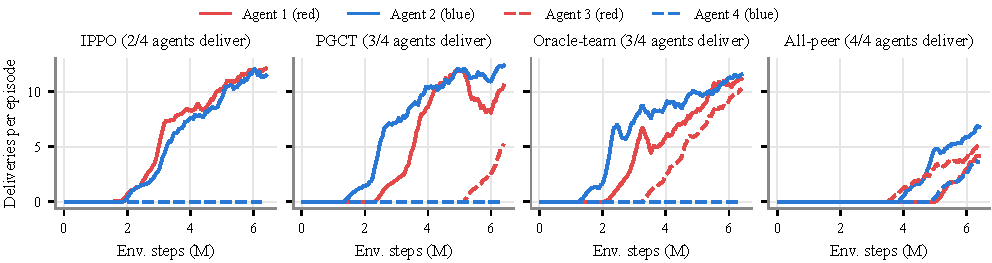
\includegraphics[width=\textwidth]{figures/fig2_per_agent_deliveries.pdf}
\caption{E1에서 agent별 episode당 배송(5점 이동평균, seed 1개). 빨강: 빨강 팀(agent 1, 3), 파랑: 파랑 팀(agent 2, 4), 실선:
agent 1--2, 점선: agent 3--4.}
\end{figure}
\begin{figure}[h]
\centering
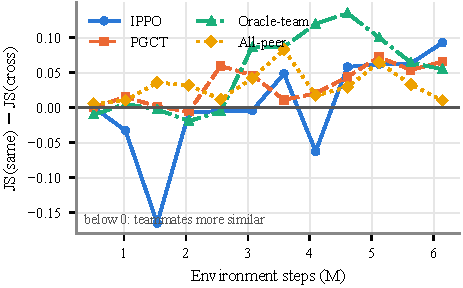
\includegraphics[width=0.6\textwidth]{figures/fig4_probe_js_gap.pdf}
\caption{E1 checkpoint에서 팀원 사이 probe divergence에서 다른 팀 agent 사이 값을 뺀 것(seed 1개). 0보다 크면 팀원이 더 다르다.
즉 실측 마진이 음수다.}
\end{figure}
\begin{figure}[h]
\centering
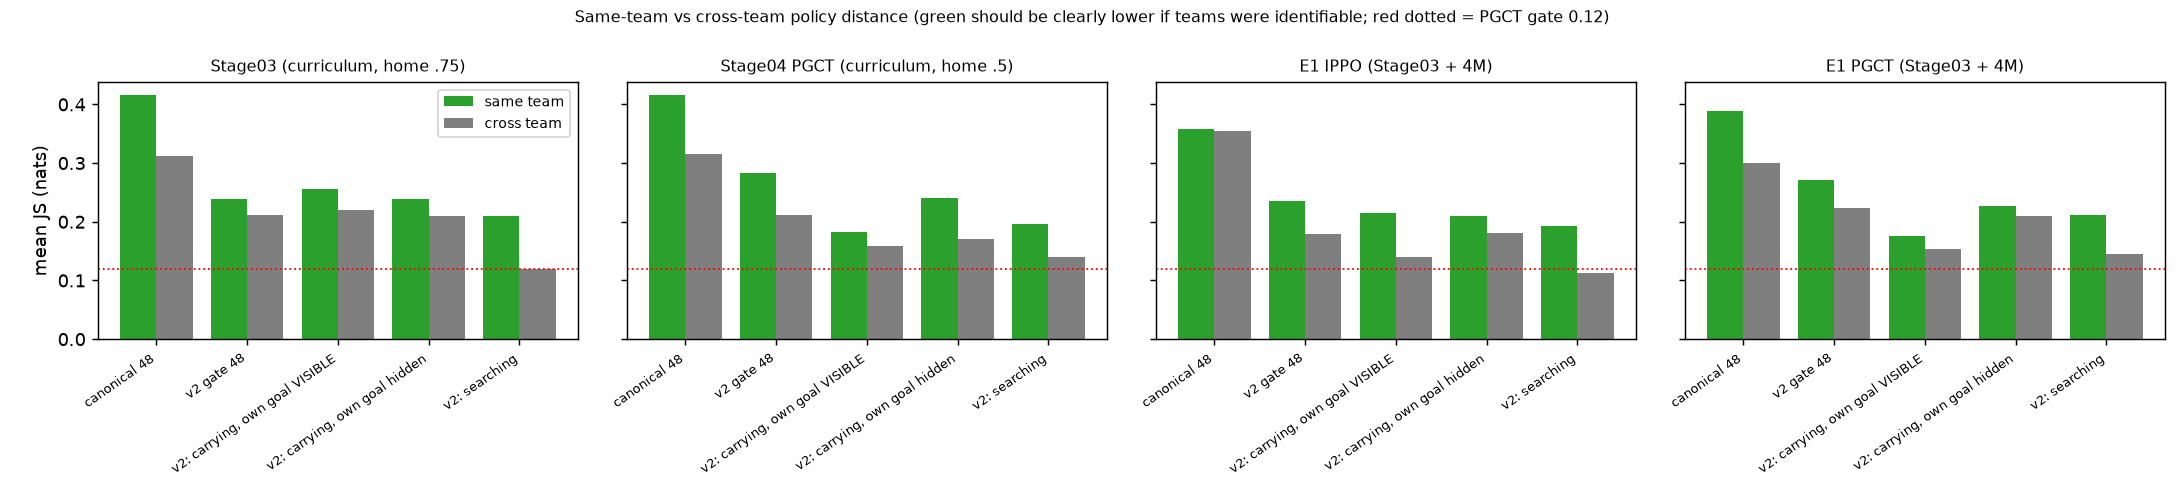
\includegraphics[width=\textwidth]{figures/frozen_probe_same_vs_cross.png}
\caption{커리큘럼 계보의 고정 E1 모델 4개와 probe 부분집합 5개(v2 추론 집합 포함)에서 팀원(초록)과 다른 팀 agent(회색) 사이 평균
probe divergence. 20개 조합 모두에서 팀원이 덜 비슷하다. 빨간 점선: $\tau=0.12$.}
\end{figure}
\begin{figure}[h]
\centering
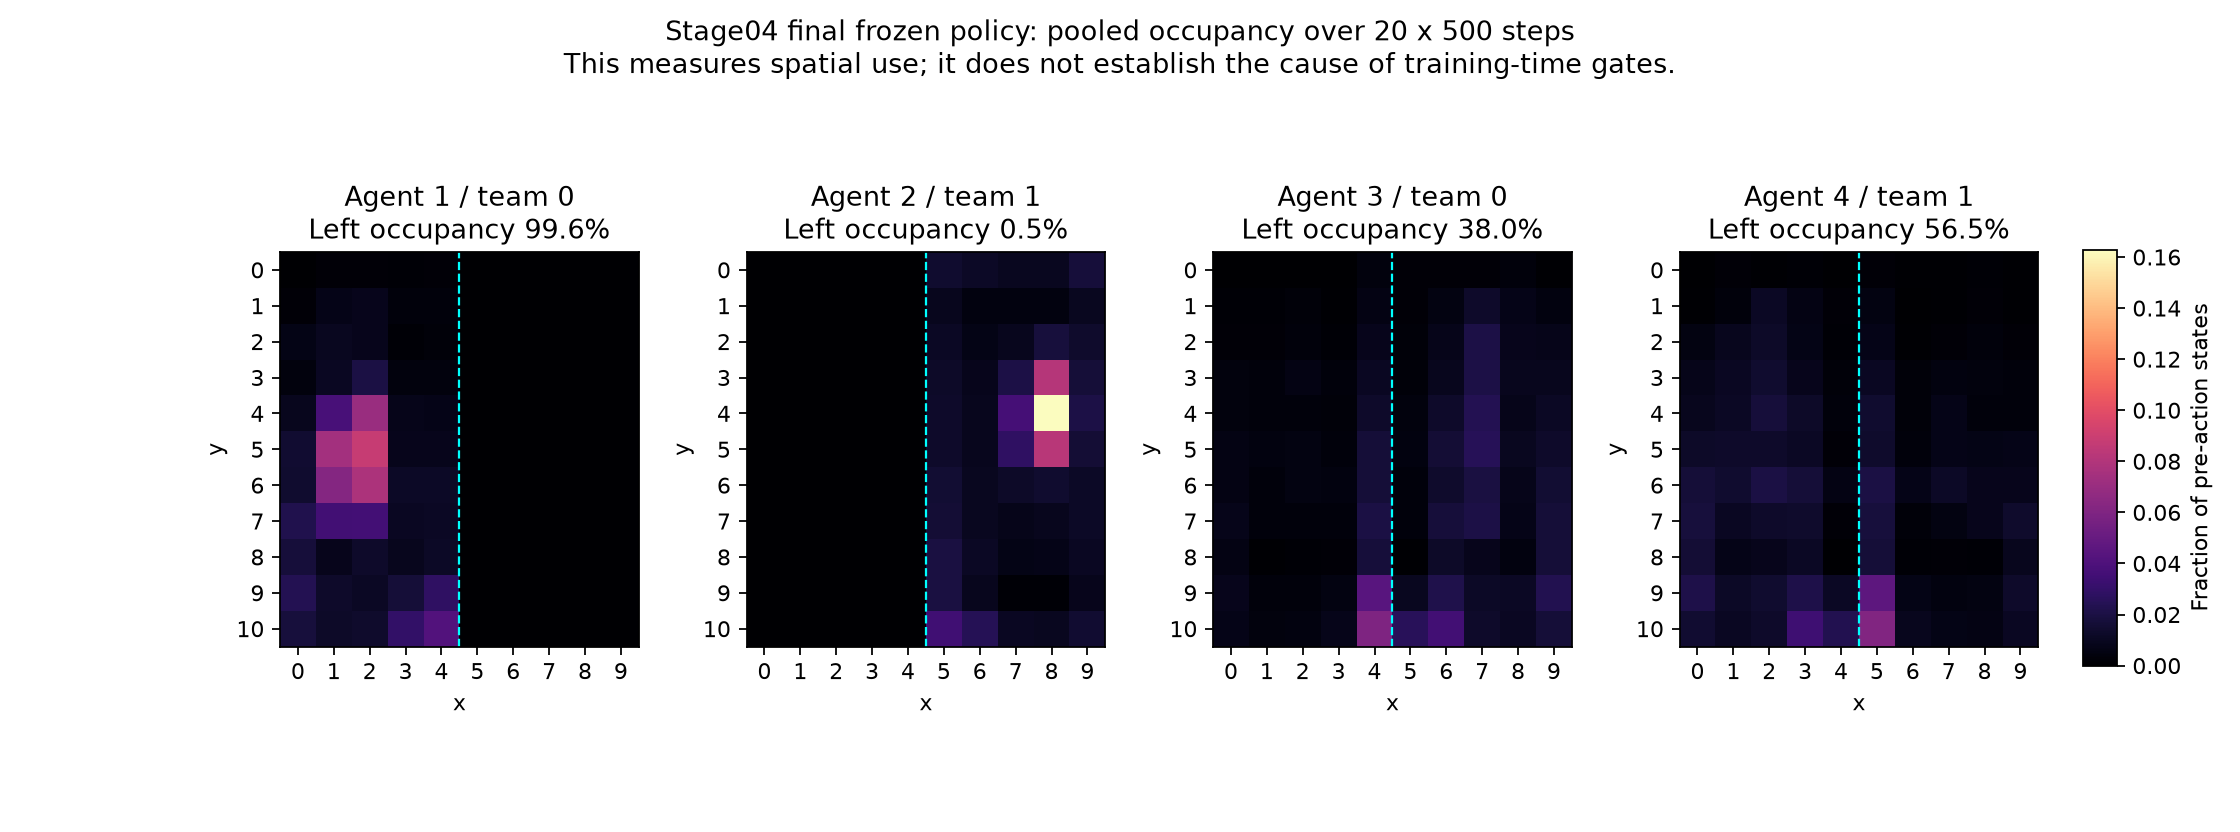
\includegraphics[width=\textwidth]{figures/stage04_occupancy.png}
\caption{고정 커리큘럼 모델의 칸별 점유(선반의 50\%가 상대 팀 쪽 절반). agent 1과 2는 자기 팀 쪽 절반에 머물고, agent 3과 4는
상대 쪽 절반에서 선반을 가져오며 gate가 가장 자주 이은 쌍이다.}
\end{figure}
\begin{figure}[h]
\centering
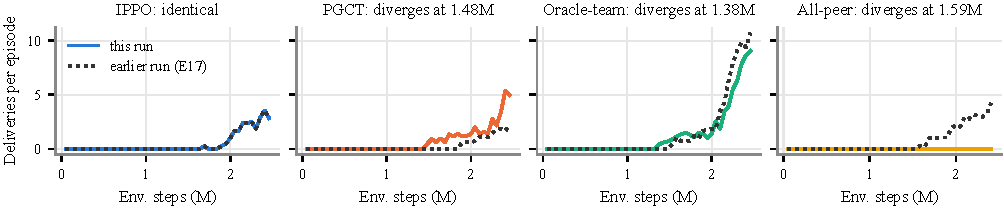
\includegraphics[width=\textwidth]{figures/figA1_reproducibility.pdf}
\caption{같은 seed와 초기 가중치의 두 실행(실선: 보고한 실행, 점선: 앞서 중단된 실행). IPPO는 정확히 재현되고, 공유 방식들은
1.4--1.6M step 이후 갈라진다.}
\end{figure}

\section{점검 세부}
\label{app:audit}
모든 점검은 고정된 가중치(전후 hash 확인)로 했고 agent 학습은 없다. 학습하거나 생성한 것은 보상 모델과 rollout뿐이다.

\textbf{모델.} 커리큘럼 계보: 1--4단계 모델(팀 선반 중 자기 쪽 절반 비율 1.0, 0.875, 0.75, 0.5)과 E1에서 이어 학습한 모델
2개(IPPO, \ours{}). 일부 분석에는 $16\times16$ 맵 모델 2개도 포함했다. 처음부터 계보: \ref{sec:e1}절의 IPPO, \ours{}, Oracle-team,
All-peer(6.4M step). 질의 창을 만든 모델은 점수에서 뺐으므로, 표~\ref{tab:audit} 창 행의 처음부터 칸은 모델 3개다.

\textbf{정책 probe.} gate와 같은 규칙(hidden 0, mask 없음, 자연로그 JS의 probe 평균)을 썼다. 규칙 기반 집합은 갈 수 있는 방향이
셋 이상인 통로 칸, 목표 비가시, 팀 상대 입력을 중립값으로 둔 상태, 목표 행에서 먼 띠로 이루어진다(상태 32개). 띠는 커리큘럼 probe를
본 뒤에 정했다. 실제 방문 창: 창 생성 정책(커리큘럼 4단계 또는 처음부터 All-peer)의 500 step episode 60개에서, 팀 라벨 없이 생성
agent들에 고르게 길이 12 창을 뽑았다. ``운반'' 창은 agent가 요청 선반을 들고 있는 창이다.

\textbf{보상 probe.} agent마다 (관측, one-hot 행동)을 입력으로 하는 MLP를, 그 모델 자신의 확률 정책으로 모은 500 step episode 20개로
초기화 seed 3개에서 학습했다. 거리는 질의 평균 $|\hat r_i-\hat r_j|$다. counterfactual 분리: 각 source episode를 reset seed와 기록된
joint action으로 재생했고(확인한 보상 3{,}804개가 모두 기록과 일치), step마다 환경을 복사한 뒤 행동한 agent의 팀을 빨강과 파랑으로
바꿔 같은 joint action을 실행했다. $Q_{\mathrm{diff}}$에서 $|r_{\mathrm{red}}-r_{\mathrm{blue}}|$의 평균은 0.002--0.051로 대부분
shaping 항이었다.

\textbf{Drift.} 자기 divergence는 두 checkpoint에서 한 agent의 응답 사이 $D$를 그 gate가 쓰는 집합에서 잰 값이다. 이것은 5 update
간격의 측정 사이 변화를 뜻하는 명제~\ref{prop:tracking}의 $\rho$가 아니다. 저장된 checkpoint로 계산할 수 있어서 보고한다
\todo{communication 기록으로 측정 간격의 $\rho$ 계산}.

\end{document}
